\documentclass[tikz,border=2]{standalone}
%% tags: spacing important tikz-qtree tree
\usetikzlibrary{shadows,arrows,shapes,positioning,calc,backgrounds,fit,automata}
\usepackage{tikz-qtree}
\begin{document}
%%%%%%%%%%%%%%%%%%%%%%%%%%%%%%%%%%%%%%%
% Define the layers to draw the diagram
\pgfdeclarelayer{bg}
\pgfsetlayers{bg,main}
%%%%%%%%%%%%%%%%%%%%%%%%%%%%%%%%%%%%%%%
% colors
\definecolor{myBlue}{HTML}{0060AD}
\definecolor{myRed}{HTML}{DD181F}
%%%%%%%%%%%%%%%%%%%%%%%%%%%%%%%%%%%%%%%

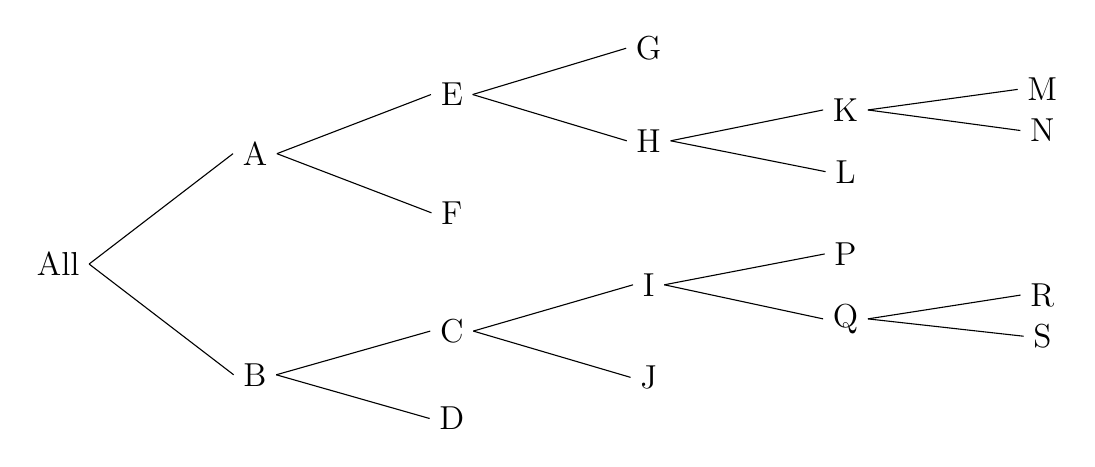
\begin{tikzpicture}[font=\large,grow'=right, sibling distance=0pt, level distance=2.5cm]
\Tree [.All 
[.A [.E G [.H [.K M N ] L ] ] F ] 
[.B [.C [.I P [.Q R S ] ] J ] D ] 
]
\end{tikzpicture}
\end{document}
